% DFG of predict() — Data Glove Review 2 (data dependencies only)
% Compile: xelatex dfg.tex
\documentclass[border=6pt]{standalone}
\usepackage{tikz}
\usetikzlibrary{shapes.geometric,arrows.meta,positioning,fit,backgrounds}

\definecolor{opfill}{HTML}{E8F0FE}
\definecolor{bb}{HTML}{F5F5F0}
\definecolor{val}{HTML}{FFF6DA}

\begin{document}
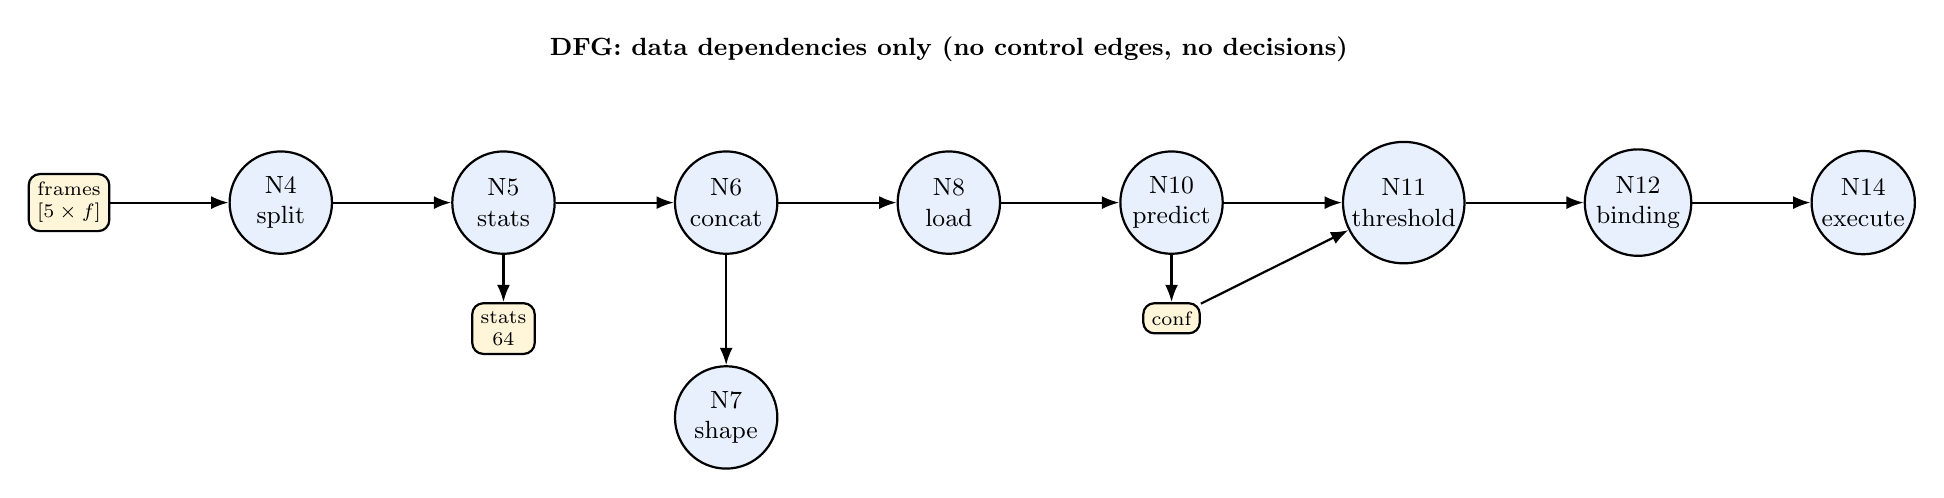
\begin{tikzpicture}[
  font=\small,
  node distance=14mm and 15mm,
  op/.style  ={circle, draw, thick, fill=opfill, minimum size=13mm, inner sep=1pt, align=center},
  val/.style ={rectangle, rounded corners, draw, thick, fill=val, inner sep=3pt, align=center, font=\scriptsize},
  data/.style={-{Latex[length=2.2mm]}, thick},
  bbstyle/.style={draw, rounded corners, fill=bb, inner sep=6pt}
]

% inputs (values)
\node[val] (frames) {frames\\$[5\times f]$};

% computation chain
\node[op, right=of frames] (n4) {N4\\split};
\node[op, right=of n4] (n5) {N5\\stats};
\node[op, right=of n5] (n6) {N6\\concat};
\node[op, below=of n6] (n7) {N7\\shape};
\node[op, right=of n6] (n8) {N8\\load};
\node[op, right=of n8] (n10) {N10\\predict};
\node[op, right=of n10] (n11) {N11\\threshold};
\node[op, right=of n11] (n12) {N12\\binding};
\node[op, right=of n12] (n14) {N14\\execute};

% value nodes
\node[val, below=6mm of n5] (vstats) {stats\\$64$};
\node[val, below=6mm of n10] (vconf) {conf};

\draw[data] (frames) -- (n4);
\draw[data] (n4) -- (n5);
\draw[data] (n5) -- (n6);
\draw[data] (n5) -- (vstats);
\draw[data] (n6) -- (n7);
\draw[data] (n6) -- (n8);
\draw[data] (n8) -- (n10);
\draw[data] (n10) -- (vconf);
\draw[data] (n10) -- (n11);
\draw[data] (vconf) -- (n11);
\draw[data] (n11) -- (n12);
\draw[data] (n12) -- (n14);

\node[above=10mm of n8, font=\small\bfseries] {DFG: data dependencies only (no control edges, no decisions)};
\end{tikzpicture}
\end{document}
